% !TEX root = ../latexnote.tex
\chapter{表格}\label{chap:table}

\section{基本表格}\label{sec:basic-table}

表格和图片类似,也有一个浮动体环境为table。

表格最基本的环境为tabular,用法如下:
\begin{lstlisting}
\begin{tabular}[可选参数]{|c|c|c|}
\hline
第一列 & 第二列 & 第三列 \\
\hline
1 & 2 & 3 \\
4 & 5 & 6 \\
\hline
\end{tabular}
\end{lstlisting}

其中\lstinline{|c|c|c|}是列格式标记,详细见\ref{sec:liegeshi},c表示列居中,|表示列之间有竖线。使用\&用来分割列,使用\lstinline|\\|表示换行。\lstinline{\hline}用来绘制行之间的横线。

\subsection{修改表格线}\label{sec:modify-table-line}
可在tabular环境外修改全部表格线的粗细,如\lstinline|\setlength{\arrayrulewidth}{2pt}|或\lstinline{\arrayrulewidth=2pt}。

如果需要单独修改表格线,可采用如下方法:

1)修改垂直表格线,使用array宏包提供的新列格式选项定义命令:
\begin{lstlisting}
\newcolumntype{新选项名称}[参数数量]{列格式}
\newcolumntype{I}{!{\vrule width 2pt}}
\end{lstlisting}
\begin{codeshow}
    \centering
    \newcolumntype{I}{!{\vrule width 2pt}}
    \begin{tabular}{|cIcIc|}
        \hline
        \multicolumn{3}{IcI}{垂直线粗细更改} \\
        \hline
        7 & 5 & 3                     \\
        \hline
        6 & 1 & 8                     \\
        \hline
    \end{tabular}
\end{codeshow}

2)修改水平表格线,可使用booktabs宏包,该宏包可以任意修改水平线粗细,还可以在上下附加一段垂直空白。

\begin{codeshow}
    \centering
    \begin{tabular}{|c|c|c|}
        \hline
        \multicolumn{3}{|c|}{水平表格线粗细更改} \\
        \specialrule{2pt}{0pt}{0pt}
        7 & 5 & 3                       \\
        \hline
        6 & 1 & 8                       \\
        \hline
    \end{tabular}
\end{codeshow}

\subsection{列格式}\label{sec:column-format}
\label{sec:liegeshi}

基本列格式如下表所示:

\begin{table}[htp]
    \centering
    \caption{\LaTeX{} 表格列格式}\label{tbl:table-column-spec}
    \begin{tabular}{*{2}{l}}
        \hline
        \textbf{列格式} & \textbf{说明}            \\
        \hline
        l/c/r        & 单元格内容左对齐/居中/右对齐,不折行    \\
        p\{width\}   & 单元格宽度固定为 {width},可自动折行 \\
        |            & 绘制竖线                   \\
        @\{string\}  & 自定义内容 {string}         \\
        \hline
    \end{tabular}
\end{table}

格中每行的单元格数目不能多于列格式里 l/c/r/p 的总数(可以少于这个总数),否则出错。

@ 格式可在单元格前后插入任意的文本,但同时它也消除了单元格前后额外添加的间距。@格式可以适当使用以充当“竖线”。特别地,\lstinline|@{}| 可直接用来消除单元格前后的间距。

另外\LaTeX{} 还提供了简便的将格式参数重复的写法 \lstinline|*{⟨n⟩}{⟨column-spec⟩}|,比如以下两种写法是等效的:
\begin{lstlisting}
    \begin{tabular}{|c|c|c|c|c|p{4em}|p{4em}|}
    \begin{tabular}{|*{5}{c|}*{2}{p{4em}|}}
\end{lstlisting}


\subsection{列宽}\label{sec:column-width}

\LaTeX{} 本身提供了 tabular* 环境用来排版定宽表格,但是不太方便使用,比如要用到 @ 格式插入额外命令,令单元格之间的间距为 \lstinline{\fill},但即使这样仍然有瑕疵:

\begin{codeshow}
    \begin{tabular*}{14em}%
        {@{\extracolsep{\fill}}|c|c|c|c|}
        \hline
        A & B & C & D \\ \hline
        a & b & c & d \\ \hline
    \end{tabular*}
\end{codeshow}

tabularx 宏包为我们提供了方便的解决方案。它引入了一个 X 列格式,类似 p 列格式,不过会根据表格宽度自动计算列宽,多个 X 列格式平均分配列宽。X 列格式也可以用 array 里的辅助格式修饰对齐方式:

\begin{codeshow}
    % \usepackage{array,tabularx}
    \begin{tabularx}{14em}%
        {|*{4}{>{\centering\arraybackslash}X|}}
        \hline
        A & B & C & D \\ \hline
        a & b & c & d \\ \hline
    \end{tabularx}
\end{codeshow}

\subsection{行距}\label{sec:row-spacing}

修改参数 \lstinline{\arraystretch} 可以得到行距更加宽松的表格:
\begin{lstlisting}
    \renewcommand\arraystretch{1.8}
\end{lstlisting}

另一种增加间距的办法是给换行命令 \lstinline|\\| 添加可选参数,在这一行下面加额外的间距,适合用于在行间不加横线的表格:


\subsection{表格标题}\label{sec:table-title}

表格标题可以用\lstinline{\caption}命令设置,默认只能在浮动体环境内部使用。

也可以在导言区添加如下命令,在浮动体外使用\lstinline{\figcaption}和\lstinline{\tabcaption}为图表添加标题。为了防止标题和图表不在一页,可以使用minipage环境将它们包起来。

\begin{lstlisting}
    \makeatletter
    \newcommand\figcaption{def\@captype{figure}\caption}
    \newcommand\tabcaption{def\@captype{table}\caption}
    \makeatother
\end{lstlisting}



\section{复杂表格}\label{sec:complex-table}

\subsection{合并单元格}\label{sec:merge-cell}

1)跨列

使用\lstinline{\multicolumn}命令可以合并列:
\begin{lstlisting}
    \multicolumn{合并列数目}{列格式}{内容}
\end{lstlisting}

2)跨行

跨行需要引入multirow宏包,使用\lstinline{\multirow}命令:
\begin{lstlisting}
    \multirow{合并行数目}{宽度}{内容} %宽度可以填*以使用自然宽度
\end{lstlisting}

既跨行又跨列时,需要把\lstinline{\multirow}命令放在\lstinline{\multicolumn}命令内部。

\begin{codeshow}
    \centering
    \begin{center}
        \begin{tabular}{|c|c|c|}
            \hline
            \multirow{2}{2cm}{A Text!}
                                     & ABC & DEF \\
            \cline{2-3}              & abc & def \\
            \hline
            \multicolumn{2}{|c|}
            {\multirow{2}*{Nothing}} & XYZ       \\
            \multicolumn{2}{|c|}{}   & xyz       \\
            \hline
        \end{tabular}
    \end{center}
\end{codeshow}

\section{问题}

\subsection{longtable与arydshln宏包冲突}\label{subsec:longtable-arydshln-conflict}
\qaq{问题:}最近帮人debug,使用longtable排版报错。
\begin{figure}[!h]
    \centering
    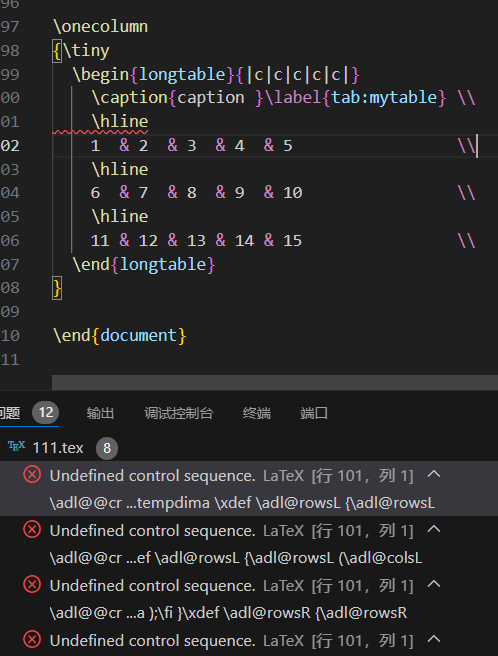
\includegraphics[width=0.4\textwidth]{figure/chap-tab/ary1.png}
    \caption{报错信息}
\end{figure}

\qaq{解决方法:}参考\href{https://zhuanlan.zhihu.com/p/667681242}{LaTeX:arydshln与longtable的冲突及教训 - 知乎 (zhihu.com)}, 发现longtable与arydshln宏包存在冲突,arydshln宏包重定义了\lstinline{\hline},可以采用如下解决方法:
\begin{enumerate}
    \item 注释掉\lstinline|\usepackage{arydshln}|。
    \item 将\lstinline|\usepackage{arydshln}|放于\lstinline|\usepackage{longtable}|之后
\end{enumerate}